\documentclass{article} 
\oddsidemargin=-5mm
\evensidemargin=-5mm\marginparwidth=.08in \marginparsep=.01in
\marginparpush=5pt\topmargin=-15mm\headheight=12pt
\headsep=25pt
\footskip=30pt
\textheight=25cm
\textwidth=17cm
\columnsep=2mm
\columnseprule=1pt\parindent=15pt\parskip=2pt

\usepackage[czech]{babel}
\usepackage[utf8]{inputenc}
\usepackage[T1]{fontenc}
\usepackage{amsmath}
\usepackage{tabularx}
\usepackage{caption}
\usepackage{ragged2e}
\usepackage{booktabs}
\usepackage{subfig}
\usepackage{float}
\usepackage{graphicx}

\begin{document}
	
\begin{center}
\bf Semestrální projekt MI-PDP 2016/2017:\\[5mm]
    Paralelní algoritmus pro řešení problému bisekční šířky\\[5mm] 
       Martin Holoubek\\[2mm]
magisterské studium, FIT ČVUT, Thákurova 9, 160 00 Praha 6\\[2mm]
18. dubna 2017
\end{center}

\section{Definice problému}
Nalezněte rozdělení množiny uzlů $V$ do dvou disjunktních podmnožin $X$, $Y$ tak, že množina $X$ obsahuje $k$ uzlů, množina $Y$ obsahuje $n-k$ uzlů a počet všech hran $\{u,v\}$ takových, že $u$ je z $X$ a $v$ je z $Y$ (čili velikost hranového řezu mezi $X$ a $Y$), je minimální.

\section{Popis sekvenčního algoritmu}
Hledání minimální bisekční šířky na obecném grafu je $\mathcal{NP}$ - těžká úloha, což nás nutí ke generování a ozkoušení všech možností. Protože musíme zkoušet všechny možné množiny uzlů o zadané velikosti, je celkový počet ozkoušených možností $\binom{n}{k}$. Kde $n$ je celkový počet uzlů a $k$ je zadaná velikost podmnožiny. Z podstaty problému vyplývá, že smysl má řešit pouze úlohy, kde $n< \lceil \frac{n}{2} \rceil$. Opačný případ je přímo převoditelný na menší problém $k_{new}=n-k$ s tím, že obě množiny ve výsledku prohodíme.


Pro výpočet minimální bisekční šířky musíme generovat jednotlivá kombinační čísla. Tyto hodnoty označují indexy uzlů náležejících do množiny $X$, zbytek uzlů grafu náleží do $Y$. Pro každé vygenerované kombinační číslo musíme spočítat počet hran mezi oběma množinama. Tímto postupem zjistíme nejmenší požadovaný počet hrany a tím pádem bisekční šířku.

Jako vylepšení hrubého přístupu jsem zvolil prořezávání stavového prostoru. To lze provést díky tomu, že při průchodu do hloubky postupně zlepšujeme odhad nejlepšího řešení. Při generování dalších kombinací tak můžeme odhadnout, současný stav algoritmu, může dostáhnout lepšího řešení. 

\subsection{Spodní mez pro prořezávání}
Pokud máme pole o velikosti $k$, ve kterém je $i$ vyplněných indexů, tak z definice množina $X$ obsahuje právě tyto uzly s těmito čísly.  Množina $Y$ obsahuje uzly s indexy, které nejsou v $X$ a jsou menší než combination[$i$]. Všechny ostatní uzly mají příslušnost neurčenou. Ta bude přidělena v dalších zanořeních algoritmu. V každém kroku spočítáme počet hran vedoucích mezi množinami a pokud toto číslo přesáhne nejlepší nalezené řešení, tuto kombinaci zahazujeme. Z rozbory problému totiž plyne, že přidání dalšího uzlu z množiny nerozhodnutých může počet hran pouze zvýšit, čímž bychom porušili minimalizu řešení.

\subsection{Implementace}
Jako implementační prostředí jsem zvolil jazyk C++ 17 kompilované pomocí překladače llvm/Clang.

Po načtení grafu z externího souboru si vygeneruji množinu hran, která obsahuje indexy uzlů, mezi jimiž daná hrana vede. Toto řešení zrychluje výpočet spodní meze a celkové bisekční šířky, protože právě tyto dvě funkce jsou pro rychlost kritické.

Samotné generování kombinačních čísel probíhá v poli o délce $k$, pomocí rekurzivního algoritmu, který generuje řešení průchodem do hloubky. Vždy, když algoritmus dojde do úrovně $k-1$, následuje spočítání hran a případný update nejlepšího nalezeného řešení. Druhou možnou implementací by bylo bitové pole, kde jednotlivé nastavení bitů by označovalo příslušnost uzlů do jednotlivých množin. Z implementačních důvodů jsem však zvolil reprezentaci polem indexů.

\subsection{Měření}
Veškeré měření probíhalo na serveru \textbf{star.fit.cvut.cz}, jehož runtime umožňuje plánování úloh tak, aby jejich běhy byly nezávislé.


\begin{center}
\begin{tabular}{l|*{6}{r}}
	vstup $\backslash$ $k$ & 5 & 7 & 10 & 15 & 16 & 17 \\
	\hline
	graph30\_7.txt & 0.01 & 0.05 & 0.61 & 1.94 & 1.79 & 1.58  \\
	graph40\_5.txt & 0.03 & 0.11 & 1.40 & 14.83 &  21.14 & 26.27  \\
	graph40\_6.txt & 0.04 & 0.19 & 3.95 & 84.30 &  130.06 & 178.70  \\
	graph50\_6.txt & 0.18 & 1.58 & 69.57 & 6186.00 &  > 7200 & xxx  \\
\end{tabular}
\captionof{table}{Naměřené časy (\textbf{s}) pro různé instance sekvenčního řešení.}
\label{table:serial}
\end{center}

Tabulka \ref{table:serial} zobrazuje délku výpočtu v závislosti na zvoleném grafu a hodnotě $k$. Pro vstupní data 30\_7 dochází u větších hodnot paradoxně ke zrychlení, které je ale způsobené symetrií problému, který se tak stane jednodušším. Pro graf 50\_6 se všechny hodnoty nepodařily naměřit a program byl po cca dvou hodinách ukončen.

\section{Popis paralelního algoritmu a implementace v OpenMP}
Zadaný problém je vhodný k paralelizaci. Výpočet jednotlivých hodnot kombinačních čísel je na sobě totiž datově nezávislý. Pro usnadnění paralelizace jsme používali knihovnu OpenMP. Abychom měli co paralelizovat je nutné vygenerovat nějaká vstupní data. 

Algoritmus pro výpočet vstupních dat je totožný s rekurzivním postupem v sekvenčním řešení. Jediný rozdíl je, že při dosažení určité konstatní hlouby je část kombinačního číslo uložena do fronty a následuje backtrack.

Po vygenerování nastupuje samotná paralelní část. OpenMP umožňuje několik způsobů paralelizace od sekcí, tasků až po datovou paralelizaci.

\subsection{Paralelizace pomocí tasků}
Hlavní paralelní smyčka vytvoří pracovní vlákna, jejichž počet je uživatelsky konfigurovatelný. Hlavní vlákno postupně bere ze smyčky vygenerované ůlohy a spouští jednotlivé paralelní tasky. Protože v programu hlídám počet vygenerovaných úloh, není nutné jejich počet omezovat. Vytvořené tasky jsou runtime systémem přidány do systémové fronty a odtud distribuovány pracovním vláknům.

Rekurzivní algoritmus je téměř totožný se sekvenčním, kromě jedné přidané kritické sekce, která zaručuje synchronizovaný přístup k proměnné globálního optima.

Po hlavním cyklu, který předává úlohy OpenMP musí následovat \textbf{taskwait}, aby hlavní vlákno počkalo na dokončení všech problémů a program se předčasně neukončil. Pro ulehčení nepoužívám rekurzivní paralelizaci, ale předgenerování úkolů, protože v další části úlohy tyto části použiji.

Výsledný program přijímá 3 parametry: datový soubor s grafem, velikost množiny $k$ a počet vláken.

\subsection{Datová paralelizace cyklem}
Protože předgenerované úlohy jsou na sobě nezávislé můžeme program paralelizovat pomocí direktivy \textbf{parallel for}. Zbytek programu probíhá totožně tako v předchozí části. Chování programu je z toho důvodu téměř totožné, dokonce i syntaxe příkazové řádky se shodná.

Konstanty, ovlivňující běh programu, jsou v obou případech shodné. Jde o hloubku předgenerovaného kombinačního čísla, které přímo ovlivňuje počet vygenerovaných úloh. Suma tasků také závisí na velikosti grafu a zadané množiny $X$. Experimentální cestou jsem pro běžné grafy s cca 40 uzly určil hloubky 4 až 5, kdy jsou výsledkem desetitisíce úloh. Tato granularita umožňuje paralelnímu algoritmu efektivní vyvažování rozdílné zátěže, která je způsobena zejména prořezáváním grafu.

\section{Popis paralelního algoritmu a implementace v OpenMPI}
Naším úkolem bylo úlohu dále paralelizovat pro systémy s distribuovanou pamětí pomocí posílání zprát. Paralelizace v OpenMPI je tak logickým rozšířením té původní pomocí OpenMP. Nám přidělenou variantu bylo za úkol zapalelizovat způsobem master - slave, kde master je hlavní proces, který řídí ostatní slavy a sám se neúčastní výpočtu.

Abychom plně využili architekturu stroje star, musíme znát jeho topologii. Ta je následující: 6 nodů, propojených pomocí sítě infiniband a ethernet. Každý z nodů obsahuje 2 sockety (CPU), přičemž každé CPU má 10 jader a navíc má podporu pro hyperthreading. Nyní můžeme rozhodnout o rozložení problému mezi výpočetní uzly. Celý problém rozložíme na master proces a 6 slave procesů, celkem tedy $N+1$, kde $N$ je počet nodů. Procesů je víc než uzlů proto, že master bude mít za úkol pouze komunikaci a rozdělování práce, tudíž obsadí pouze jedno jádro, zbývající proces tedy obsadí zbylá jádra.

\subsection{Implementace}
Aby všechny procesy mohly provádět výpoče nad stejným grafem, je nutné ho v hlavním procesu načíst a rozeslat dále. Toho lze dosáhnout pomocí broadcastu, případně opakovaného unicastu. Protože se jedná o paralelizaci typu master a slave, úlohy pro ostatní procesy vygeneruje hlavní process (v OpenMPI značený rankem $0$). Tyto úlohy jsou generovány totožně jako v paralelním řešení pomocí OpenMP a jsou uloženy ve frontě hlavního procesu. Výpočetní procesy, které jsou již spuštěny pošlou požadavkem na práci a čekají, až hlavní proces napočítá a odešle část práce. 

Pro zefektivnění procesu jsou úlohy odesílány v balících, jejichž velikost je konstantní. Abychom využili potenciál stroje star, na každém výpočetním uzlu spustíme pomocí OpenMP několik vláken. Tato vlákna jsem paralelizoval direktivou \textbf{parallel for}, cyklus beze úlohy přímo z hlavní fronty a jde tak o přímočaré řešení. Výpočty probíhají dokud nejsou vyčerpána fronta úkolu v hlavním procesu. Ten pak rozešle broadcast všem slavům, ve kterém žádá o lokální maxima. Po odeslání řešení se slave procesy ukončí a hlavní proces spočítá hodnotu bisekční šířky z přijatých dat, poté se i on ukončí.

Stejně jako při paralelizaci je zásadním parametrem počet předpočítaných úkolů. Latence sítě by totiž mohla negativně ovlivlit čas řešení pokud bychom počet přehnali. Druhým parametrem na němž závisí rychlost komunikace je počet úkolu, které se najednou odešlou slave uzlu. Experimentálním vyhodnocením jsem došel k závěru, že je rozumné předpočítat si desítky tisíc úkolů a ty distribuovat po stovkách.

Možným zlepšením programu by byla úvodní fáze. Mohli bychom rozeslat graf všem uzlů a nechat je všechny předpočítat úlohy. Za předpokladu symetrického systému by tato fáze měla trvat stejně dlouho jako nyní, protože výpočty by běžely nezávisle. Nyní by přidělení úkolu neznamenalo odeslat $k*CNT$ čísel, ale pouze dva indexy do tabulky předpočítaných startů. Ušetřili bychom tím síťovou komunikaci, na druhou stranu by toto řešení zbytečně spotřebovávalo pamět jednotlivých uzlů.

\newcommand{\mc}[1]{\multicolumn{2}{r|}{#1}}
\section{Naměřené výsledky a vyhodnocení}

\begin{center}
\begin{tabular}{l|rrrrrrr}
	threads	& 1 & 2 & 4 & 8 & 16 & 24 & 32  \\ 
	\hline
	Serial 		& \multicolumn{7}{c}{356.00} \\ 
	OpenMP task & 362.28 & 206.83 & 102.58 & 56.43 & 32.21 & 29.04 & 24.63 \\ 
	OpenMP loop & 405.71 & 207.92 & 106.27 & 67.04 & 66.59 & 56.84 & 43.13 \\
\end{tabular} 
	\captionof{table}{Naměřené časy (\textbf{s}) paralelních řešení pro data40\_6.txt, $k$ = 19}
	\label{table:parallel1}
\end{center}

\begin{center}
	\begin{tabular}{l|rrr}
	procs x thrs	& 1 & 2 & 4 \\
	\hline
	1 & 384.40 & 227.50 & 127.00 \\
	4 & 182.50 & 106.50 & 59.58 \\
	8 & 98.10 & 48.40 & 24.50 \\
	16 & 51.00 & 9.93 & 16.10 \\
	24 & 42.00 & 27.40 & 9.32 \\
	32 & 29.00 & 12.38 & 6.10 \\
	\end{tabular} 
	\captionof{table}{Naměřené časy (\textbf{s}) řešení v OpenMPI pro data40\_6.txt, $k$ = 19}
	\label{table:parallel2}
	\begin{figure}[H]
		\centering
		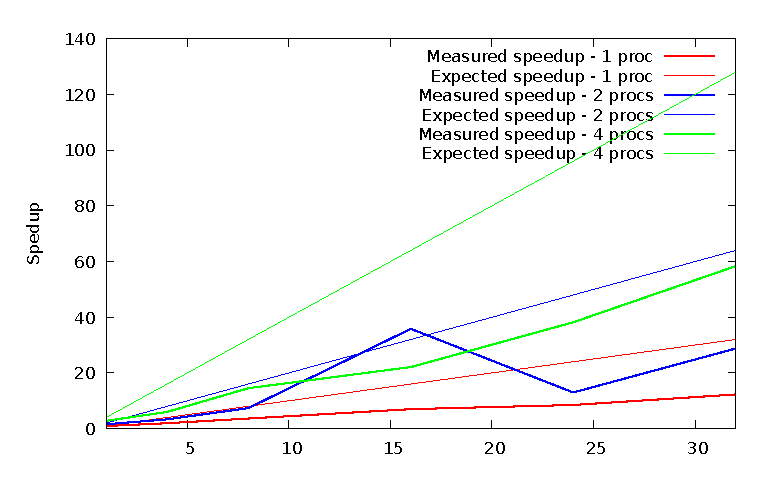
\includegraphics{mpi_speedup_19_graph40_6.eps}
		\caption{Naměřené zrychlení řešení v OpenMPI pro data40\_6.txt, $k$ = 19}%
	\end{figure}
\end{center}

\begin{center}
\begin{tabular}{l|rrrrrrr}
	threads	& 1 & 2 & 4 & 8 & 16 & 24 & 32  \\ 
	\hline
	Serial 		& \multicolumn{7}{c}{44.17} \\ 
	OpenMP task & 46.16 & 21.56 & 9.51 & \textbf{3.72} & 4.63 & 3.61 & 3.08 \\ 
	OpenMP loop & 45.99 & 23.86 & 9.75 & 6.12 & 5.98 & 5.82 & 4.83 \\
\end{tabular} 
\captionof{table}{Naměřené časy (\textbf{s}) paralelních řešení pro data40\_5.txt, $k$ = 19}
\label{table:parallel3}
\end{center}


\begin{center}
	\begin{tabular}{l|rrr}
		procs x thrs	& 1 & 2 & 4 \\
		\hline
		1 & 45.49 & 24.75 & 15.06 \\
		4 & 16.52 & 10.59 & 6.25 \\
		8 & 7.01 & 4.29 & 3.43 \\
		16 & 3.25 & 2.98 & 2.76 \\
		24 & 1.99 & 2.29 & \textbf{1.17} \\
		32 & 1.42 & 1.97 & 1.03 \\
	\end{tabular} 
	\captionof{table}{Naměřené časy (\textbf{s}) řešení v OpenMPI pro data40\_5.txt, $k$ = 19}
	\label{table:parallel4}
		\begin{figure}[H]
		\centering
		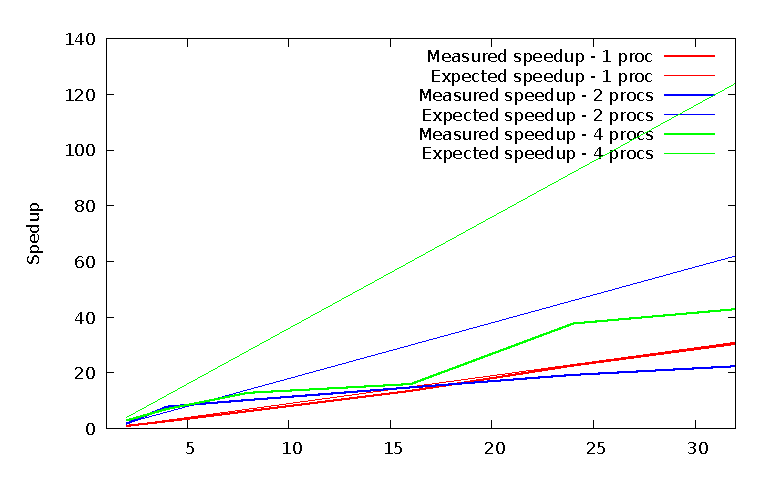
\includegraphics{mpi_speedup_19_graph40_5.eps}
		\caption{Naměřené zrychlení řešení v OpenMPI pro data40\_5.txt, $k$ = 19. Všimněte si superlineárního zrychlení pro jedno vlákno.}%
	\end{figure}
\end{center}


\begin{center}
\begin{tabular}{l|rrrrrrr}
	threads	& 1 & 2 & 4 & 8 & 16 & 24 & 32  \\ 
	\hline
	Serial 		& \multicolumn{7}{c}{260.67} \\ 
	OpenMP task & 268.35 & 122.95 & 68.31 & \textbf{27.78} & 19.03 & 15.67 & 15.24 \\ 
	OpenMP loop & 260.69 & 132.80 & 68.11 & 35.53 & 19.75 & 17.11 & 15.20 \\
\end{tabular} 
\captionof{table}{Naměřené časy (\textbf{s}) paralelních řešení pro data50\_6.txt, $k$ = 11}
\label{table:parallel5}
\end{center}


\begin{center}
	\begin{tabular}{l|rrr}
		procs x thrs	& 1 & 2 & 4 \\
		\hline
		1 & 231.25 & 126.43 & 67.89 \\
		4 & 80.50 & 48.25 & 22.68 \\
		8 & 42.28 & \textbf{13.47} & 12.32 \\
		16 & 22.72 & 11.46 & 7.64 \\
		24 & 14.91 & 8.45 & 5.47 \\
		32 & 10.08 & 5.78 & 3.45 \\
	\end{tabular} 
	\captionof{table}{Naměřené časy (\textbf{s}) řešení v OpenMPI pro data50\_6.txt, $k$ = 11}
	\label{table:parallel6}
		\begin{figure}[H]
		\centering
		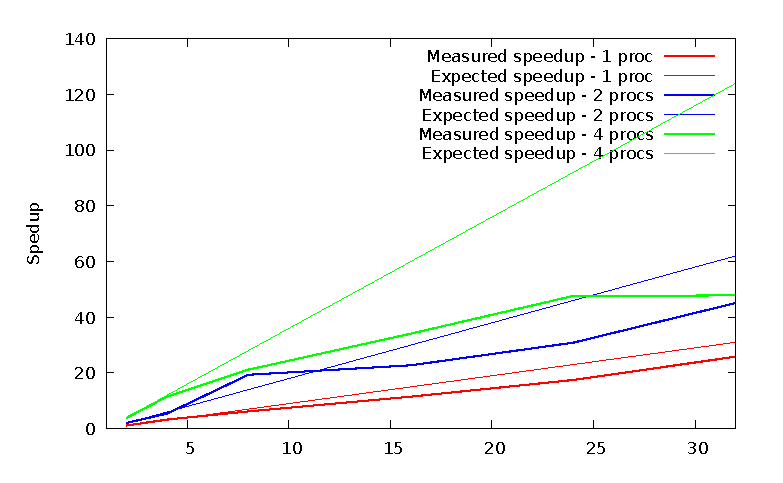
\includegraphics{mpi_speedup_11_graph50_6.eps}
		\caption{Naměřené zrychlení řešení v OpenMPI pro data50\_6.txt, $k$ = 11. Všimněte si superlineárního zrychlení pro 2 vlákna.}%
	\end{figure}
\end{center}

\section{Závěr}
Během implementace úkolů jsem se seznámil s teoretickou i praktickou částí paralelního programování pro platformy OpenMP a OpenMPI. Z grafů je vidět, že mé řešení relativně hezky škáluje s rostoucím počtem procesůrů i vláken. Většinou je zrychlení téměř lineární. V několika případech se dostavilo superlineární zrychlení, které je způsobenou náhodnou distribucí práce jednotlivým uzlům. Nalezená lokální maxima totiž ovlivňují zbytek běhu algoritmu a mohou tak vést k efektivnějšímu prořezávání a efektu superlinerního zrychlení. Toto chování je v tabulkách naznačeno \textbf{tučným písmem}.

Jako velice výhodné zlepšení se ukázala implementace globálního optima, které se rozesílá na výpočetní uzly během zasílání úloh. Takto mohou jednotlivý pracovníci efektivnějsi synchronizovat svou práci a zejména prořezávat. Výsledkem bylo rapidní zrychlení a zvášení výskyt superlineárního zrychlení.

Celkově mě semestrální práce opravdu bavila a z mého pohledu mi přinesla zajímavé zkušenosti.
\end{document}
